\documentclass[12pt]{article}
\usepackage{graphicx}
\usepackage{enumitem}
\usepackage{amsmath}
\usepackage{gvv-book}
\usepackage{gvv}

\title{\textbf{Application Problem}}
\author{\textbf{EE25BTECH11008 - Anirudh M Abhilash}}
\date{October 4, 2025}

\begin{document}

\maketitle

\section*{Question}

A fraction becomes $\frac{1}{3}$ when $1$ is subtracted from the numerator and it becomes $\frac{1}{4}$ when $8$ is added to the denominator. Find the fraction.

\section*{Solution}

Let the fraction be $\frac{x}{y}$.  

\begin{align}
\frac{x-1}{y} &= \frac{1}{3}, \\
\frac{x}{y+8} &= \frac{1}{4}
\end{align}

\begin{align}
3(x-1) - y &= 0 \implies 3x - y - 3 = 0, \\
4x - (y+8) &= 0 \implies 4x - y - 8 = 0
\end{align}

\begin{align}
(3 \ -1) \myvec{x \\ y} &= 3, \\
(4 \ -1) \myvec{x \\ y} &= 8
\end{align}

Augmented matrix:

\begin{align}
\augvec{2}{1}{3 & -1 & 3 \\ 4 & -1 & 8}
\end{align}

RREF using row operations:

\begin{align}
R_2 &\to R_2 - \frac{4}{3} R_1 \implies 
\augvec{2}{1}{3 & -1 & 3 \\ 0 & 1/3 & 4} \implies
\augvec{2}{1}{3 & -1 & 3 \\ 0 & 1 & 12}, \\
R_1 &\to R_1 + R_2 \implies 
\augvec{2}{1}{3 & 0 & 15 \\ 0 & 1 & 12} \implies
\augvec{2}{1}{1 & 0 & 5 \\ 0 & 1 & 12}
\end{align}

\begin{align}
\myvec{x \\ y} = \myvec{5 \\ 12}
\end{align}

Hence, the fraction is:

\[
\boxed{\frac{5}{12}}
\]

\begin{figure}[H]\centering
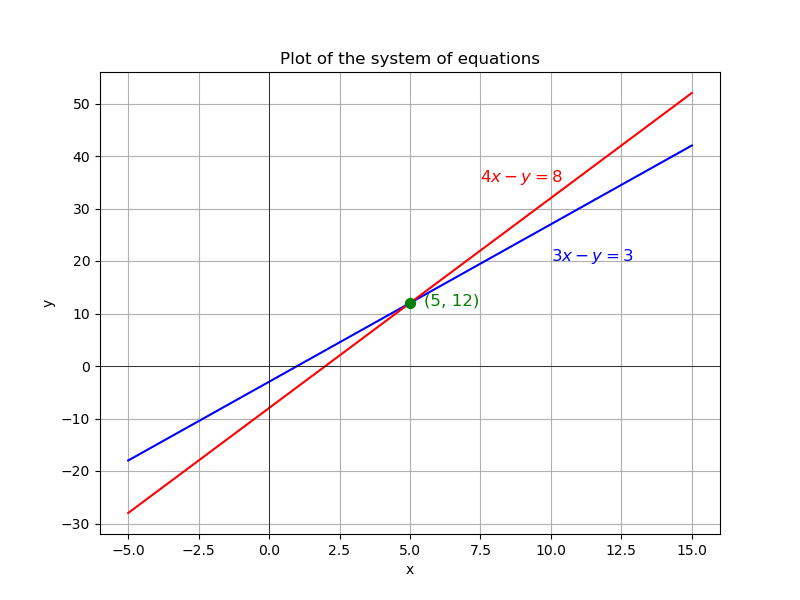
\includegraphics[width=1\columnwidth]{figs/plt.png}
\caption{Equations}
\label{fig:plt}
\end{figure}

\end{document}
